\documentclass[12pt]{article}
\usepackage{amsmath,latexsym,amsfonts,amssymb,graphicx,amsthm,epsfig,enumerate}
\usepackage{tikz,verbatim,tabularx} % adds charting fuctions
\newcolumntype{C}{>{\centering\arraybackslash}X}
\linespread{1.2}

%\pagestyle{empty}

\begin{document}
	\title{6 Man's Morris: 2AA4/2ME3 Assignment 3} %add title here
	\author{
		Gregory Smilski, 1404091\\
		Abigail Gaulin, 1327924\\
		Karl Knopf 1437217} 
	% add other necessary information here
	
	\maketitle
	\thispagestyle{empty}
	\newpage
	\tableofcontents
	\newpage
	
	\section{Introduction}
	This document describes the java project 6 Men's Morris. 
	\subsection{Architecture}
	\begin{figure}[!h]
		\centering
		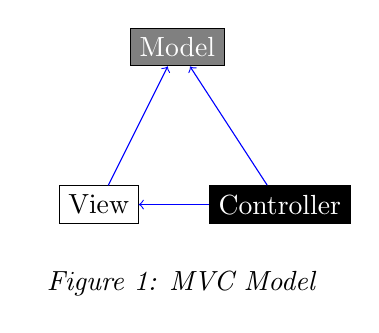
\begin{tikzpicture}
		% MVC Architecture
		\node[draw] (View) at (0,0) {View};
		\node[draw,fill=black,text=white] (Controller) at (2.3,0) {Controller};
		\node[draw,fill=gray,text=white] (Model) at (1,2) {Model};
		
		\draw[->,draw=blue] (View) to (Model);
		\draw[->,draw=blue] (Controller) to (View);
		\draw[->,draw=blue] (Controller) to (Model);
		\node at (1.0, -1.0) {\textit{ Figure 1: MVC Model}};
		
		\end{tikzpicture}
	\end{figure}
	This software uses MVC architecture in its design. MVC stands for Model, View, Controller, and is a design tool used in software development. The View contains all information the user sees, and interacts with the user. The Model contains all the data, and the Controller contains commands which modify the view and model. This architectural style is useful as it allows for modulation, and parts of the program can be modified without affecting any others.
	\subsection{Technologies}
	\begin{itemize}
		\item Java:  An object oriented programming language 
		\item Eclipse: It is an IDE used for the development and testing of software typically in Java
		\item Java Swing: A java toolkit designed to aid programmers in the creation of gui applications. This widget toolkit allows the programmer quick access to various predefined graphical objects, allowing the easy creation of a graphical interface.
		
	\end{itemize}
	\section{Modular Decomposition}
	% 4.1Description of the classes and modules and why they were used
		\begin{figure}[!h]
			\centering
			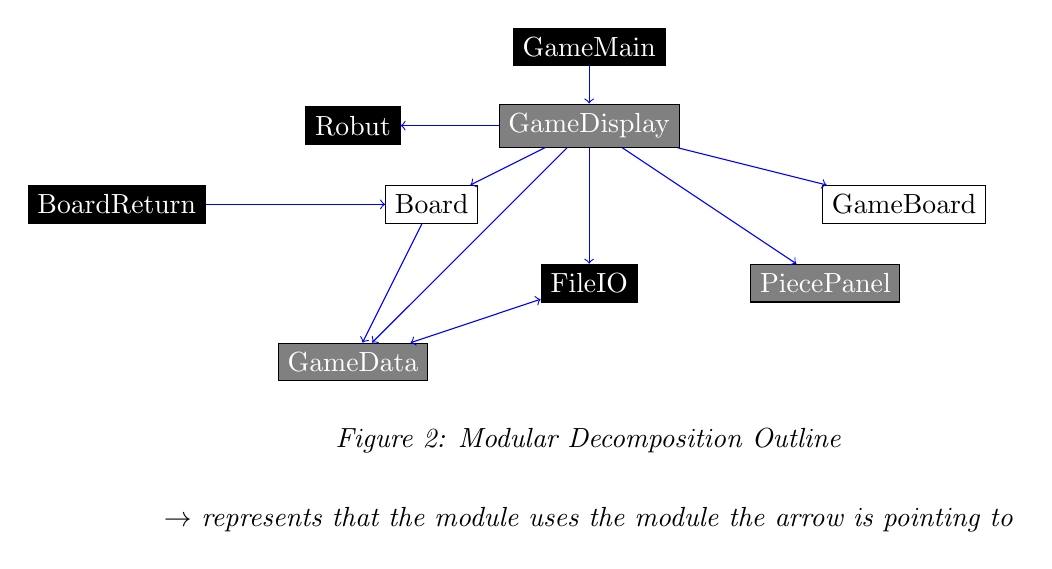
\begin{tikzpicture}
			% MVC Architecture
			\node[draw] (Board) at (-1,1) {Board};
			\node[draw,fill=white,text=black] (GameBoard) at (5,1) {GameBoard};
			\node[draw,fill=gray,text=white] (GameDisplay) at (1,2) {GameDisplay};
			\node[draw,fill=gray,text=white] (PiecePanel) at (4,0) {PiecePanel};
			\node[draw,fill=black,text=white] (BoardReturn) at (-5,1){BoardReturn};
			\node[draw,fill=black,text=white](GameMain) at (1,3) {GameMain};
			\node[draw,fill=gray,text=white] (GameData) at (-2,-1){GameData};
			\node[draw,fill=black,text=white] (FileIO) at (1,0) {FileIO};
			\node[draw,fill=black,text=white] (Robut) at (-2,2) {Robut};
			
			\draw[->,draw=blue] (GameDisplay) to (Board);
			\draw[->,draw=blue] (GameDisplay) to (PiecePanel);
			\draw[->,draw=blue] (GameDisplay) to (GameBoard);
			\draw[->,draw=blue] (BoardReturn) to (Board);
			\draw[->,draw=blue] (GameMain) to (GameDisplay);
			\draw[->,draw=blue] (GameDisplay) to (FileIO);
			\draw[->,draw=blue] (GameDisplay) to (GameData);
			\draw[->,draw=blue] (Board) to (GameData);
			\draw[->,draw=blue] (GameDisplay) to (Robut);
			\draw[<->,draw=blue] (FileIO) to (GameData);
			
			\node at (1.0, -2.0) {\textit{Figure 2: Modular Decomposition Outline  }};
			\node at (1.0, -3.0) {\textit{$\rightarrow$ represents that the module uses the module the arrow is pointing to  }};
			
			\end{tikzpicture}
		\end{figure}
	The modules chosen (as detailed in the Module Guide), were done so in order to make it straightforward for the 3 members involved in the project to code individually, and also to enforce modularity in the program. The GameDisplay, GameBoard and PiecePanel make up the View. The PiecePanel creates the tokens to take the user input, GameDisplay creates buttons to check or restart the game, and GameBoard displays the game data to the user. By dividing the View up in this way, if any of these functionalities need to be modified that can be done without affecting the other parts.\\ \emph{new} \\Board ,as well as part of GameDisplay make up the Controller.  This controls the game logic, and is called by the View to make modifications to the game data based on user input.
	It makes sense for the Controller to be separate from the other modules, as any changes that are made to the game logic can be implemented without there being any change to what the user sees/interacts with, and likewise any changes to the user interface will not interfere with the game logic/data. The class robut is also part of the controller. It manages the logic of the AI.
	\\	The model is contained in the GameData class. Here the game information is stored, and it can be used by the view and the controller. The controller is also able to update the model.
	\section{Module Guide}
	%4.2 For each module, a description of the interface and behaviors of each method
	\subsection{MIS}

	\begin{itemize}
			\item GameMain.java \\
			This module houses the main function of the program, and allows it to run. It creates a game display object the projects to the screen.\\
			\underline{Interface} \\
			\underline{Uses}
			\begin{itemize}	
				\item GameDisplay.java
				\item javax.swing.SwingUtilities;
			\end{itemize} 
			\underline{Return Type}
			\begin{itemize}
				\item None
			\end{itemize}
			\underline{Access Programs}
			\begin{itemize}
				\item public main(String args[]) : A main method that runs the program.

			\end{itemize}
		

		\item GameDisplay.java \\
		This module creates the Game Displayed to the window of the game. It controls some of logic of the game, and calls other classes to generate the game board (so it controls the view). \\
		\underline{Interface} \\
		\underline{Uses}
		\begin{itemize}
			\item Gameboard.java
			\item PiecePanel.java
			\item Board.java
			\item FileIO.java
			\item GameData.java
			\item java.awt.*
			\item javax.swing.*
			\item javax.swing.border.*
			\item java.awt.event.ActionEvent
			\item java.awt.event.ActionListener
			\item java.awt.event.MouseAdapter
			\item java.awt.event.MouseEvent
			\item java.io.*
			\item java.io.PrintWriter
			\item java.util.Random
		\end{itemize} 
		\underline{Return Type}
		\begin{itemize}
			\item None
		\end{itemize}
		\underline{Access Programs}
		\begin{itemize}
			\item public GameDisplay(String title) : A constructor for the GameDisplay class. Creates an GameDisplay object with a title, that is specified by String title. This method is necessary to allow other classes to create a game display, and run the program.
			\item public GameDisplay() :Creates an GameDisplay object, using the default settings and title. Calls the public method GameDisplay(String title) to create an instance of the Game Dispaly class.
			\item public void actionPerformed(ActionEvent e): A public method that overrides the more general actionPerformed. This method specifies the actions taken when the buttons in the button panel are used.
		\end{itemize}
		\item GameBoard.java \\
		This module contains the data and specifications for displaying the 6 man's morris board to the window. It is used by Game Display to create the full game board. \\
		\underline{Interface} \\
		\underline{Uses}
		\begin{itemize}
			\item java.awt.Color;
			\item java.awt.Graphics;
			\item java.awt.Graphics2D;
			\item java.awt.Shape; 
			\item java.awt.geom.Ellipse2D;
			\item java.awt.geom.Line2D;
			\item java.awt.geom.Rectangle2D;
			\item java.util.Random;
			\item javax.swing.JPanel;
		\end{itemize} 
		\underline{Return Type}
		\begin{itemize}
			\item None
		\end{itemize}
		\underline{Access Programs}
		\begin{itemize}
			\item public Shape[][] getShapeArray() : A public method to allow other class to access the values of the shapeArray 2D array. This allows other class to see the shape of each element on the board.
			\item public void setVisibleTeams(int i, int j, int value) : A public method to allow other classes the ability to change the values of the  visibleTeams array. This allows another class to change which player controls that space (has a piece on that space).
			\item public int getVisibleTeams(int i, int j) : A public method that allows another class to get the value of the visibleTeams array at a specified i and j value. This allows another class to see which player has a piece on that space, if any.
			\item public GameBoard() : A public constructor for the class. This allows another class to be able to create a GameBoard panel for the general display.

		\end{itemize}
			\item PiecePanel.java \\
			This module contains the data and specifications for displaying the piece panel and messages to the window. It is used by Game Display to create the full game board. \\
			\underline{Interface} \\
			\underline{Uses}
			\begin{itemize}
				\item java.awt.Color;
				\item java.awt.Graphics;
				\item java.awt.Graphics2D;
				\item java.awt.Shape; 
				\item java.awt.geom.Ellipse2D;
				\item javax.swing.JPanel;
				\item javax.swing.JLabel;
			\end{itemize} 
			\underline{Return Type}
			\begin{itemize}
				\item None
			\end{itemize}
			\underline{Access Programs}
			\begin{itemize}
				\item public Shape getRedCircle() : returns the value of RedCircle.
				\item public Shape getBlueCircle() : returns the value of BlueCircle.
				\item public void setLabel(String newText) : Allows another class to set the String message to be displayed to the screen.
				\item public void setRedCount(String newText) : Allows another class to set the amount of remaining red disks to be placed.
				\item public void setBlueCount(String newText) : Allows another class to set the amount of remaining blue disks to be placed.
				\item public PiecePanel() : A constructor that allows another class to create an instance of the PiecePanel class.
				
			\end{itemize}
			
				\item robut.java \\
				This module acts as an Artificial Intelligence to determine what move the computer should make. It is used by GameDisplay.java to give the computer’s next move based on a given board  \\
				\underline{Interface Uses} 
				\begin{itemize}
					\item none
				\end{itemize} 
				\underline{Return Type}
				\begin{itemize}
					\item Information on the game currently being played
				\end{itemize}
				\underline{Access Programs}
				\begin{itemize}
					\item public static int[] place(int[][] visibleTeams, int colour, int added) : A public method that, based on the setup of the board and the number of pieces on it, determines and returns a location on the board where a new piece should be placed.
					\item public static int[] move(int[][] visibleTeams, int colour) : A public method that, based on the setup of the board, determines and returns a set of locations on the board of what piece should be moved and where it should be moved to.
					\item public static int[] mill(int[][] visibleTeams, int colour, int added) : A public method that, based on the setup of the board determines and returns the location of a piece on the board that should be removed.
				\end{itemize}
				\item GameData.java \\
				This module acts as the module in MVC framework, and stores and returns the information for the game currently in play. It is used by GameDisplay.java and Gameboard.java to return and update game data, and by FileIO.java return game data to be saved. \\
				\underline{Interface Uses} 
				\begin{itemize}
					\item FileIO.java
				\end{itemize} 
				\underline{Return Type}
				\begin{itemize}
					\item Information on the game currently being played
				\end{itemize}
				\underline{Access Programs}
				\begin{itemize}
					\item public GameData() : A constructor for GameData class. Allows another class to create Game Data for a new game.
					\item public int[][] getVisibleTeams() : A getter method for the locations of the pieces on the game board.
					\item public void setVisibleTeams(int x, int y, int value) : A setter method for an individual value of visibleTeams. Allows a piece to be added to the gameboard.
					\item public void setVisibleTeams(int[][] newTeams) : A setter method for the whole of visibleTeams. Allows for an old game to be loaded to the game board.
					\item public void incrementPlay1count() : Increments the number of pieces played by player 1 by 1.
					\item public void decreasePlay1count() : Decrements the number of pieces played by player 1 by 1.
					\item public void setPlay1count(int count) : A setter method for the number of pieces played by player 1. Allows for an old game’s count of player 1’s pieces to be loaded.
					\item public int getPlay1count() : A getter method for the number of pieces played by player 1.
					\item public int getPlay1removed() : A getter method for the number of player 1’s pieces that were removed.
					\item public void incrementPlay2count() : Increments the number of pieces played by player 2 by 1.
					\item public void decreasePlay2count() : Decrements the number of pieces played by player 2 by 1.
					\item public void setPlay2count(int count) : A setter method for the number of pieces played by player 2. Allows for an old game’s count of player 2’s pieces to be loaded.
					\item public int getPlay2count() : A getter method for the number of pieces played by player 2.
					\item public int getPlay2removed() : A getter method for the number of player 2’s pieces that were removed.
					\item public void setRedTake(bolean value) : A setter method for whether or not red can take one of blue’s pieces.
					\item public Boolean getRedTake() : A getter method for whether or not red can take one of blue’s pieces.
					\item public void setBlueTake(bolean value) : A setter method for whether or not blue can take one of red’s pieces.
					\item public Boolean getBlueTake() : A getter method for whether or not blue can take one of red’s pieces.
					\item public void incrementTake() : A method that switches which player is active.
					\item public void setFirst(boolean bool) : A setter method that sets which player moves first.
					\item public boolean getFirst() : A getter method that returns which player moves first.
					\item public void setState(int state) : A setter method that sets the previous state to the current state and sets the current state to the new state.
					\item public int getCurrentState() : A getter method that returns the current state of the game.
					\item public int getPreviousState() : A getter method that returns the previous state of the game.
					\item public int getPreviousMoves() : A getter method that returns the number of moves previously made.
					\item public void resetPreviousMoves() : A method that sets the number of previous moves to 0.
					\item public void incrementPreviousMoves() : A method that increases the number of previous moves by 1.
					\item public void loadGame() : A method that loads a game state from a txt file.
				\end{itemize}
\item FileIO.java \\
This module saves the current game and loads the previous saved game. \\
\underline{Interface} \\
\underline{Uses}
\begin{itemize}
	\item java.io.BufferedReader
	\item java.io.File
	\item java.io.FileReader
	\item java.io.PrintWriter
\end{itemize}
\underline{Return Type}
\begin{itemize}
	\item None
\end{itemize}
\underline{Access Programs}
\begin{itemize}
	\item public static void saveGame(GameData gameData): A public method which writes the current game data to a text file, allowing the user to save their progress.
	\item public static int[][] loadGame(): A public method which reads from an exsisting text file, allowing the user to return to a saved point in a game they already started.
\end{itemize}


\item Board.java \\
This module creates the game logic, and contains the error and logic checkers for the game. \\
\underline{Interface} \\
\underline{Uses}
\begin{itemize}
	\item GameDisplay.java
	\item GameData.java
	\item Boardreturn.java
	\item javax.swing.SwingUtilities
	\item java.util.Random;
\end{itemize} 
\underline{Return Type}
\begin{itemize}
	\item None
\end{itemize}
\underline{Access Programs}
\begin{itemize}
	\item public boolean startboard(int[]][] visibleteams) : Sets up the array to keep track of piece positions on board, generates random boolean to determine which player goes first. Returns boolean (true - player1, false - player 2).
	\item public void newpiece(int l, int p, boolean teamnew, int visibleteams[]][], int play1count, int play2count): Adds new piece to array as long as there is no piece already in position and tracks how many pieces from each player have been added to board. Returns array of current board, and int value determining whether new piece position was legal (1 - legal).
	\item public Boardreturn okaymovecheck(int team) : Determines whether any piece of the inputted team is able to move. If not, returns a 0, and player looses.
	\item public static Boardreturn movepiece(int ol,int op,int nl,int np, int[][] visibleteams) : Holds values determining whether or not move/new piece placement is legal, and current array after new piece/move piece attempted. 
	\item public static int checkpiece(int oldl, int oldp, int newl, int newp, int[][] visibleteams): Checks whether proposed piece movement is legal based on current position, and position of other pieces on board.
	
\end{itemize}
\item Boardreturn.java \\
This module creates a return type to help determine if a boardstate is legal. \\
\underline{Interface} \\
\underline{Uses}
\begin{itemize}
	\item None
\end{itemize} 
\underline{Return Type}
\begin{itemize}
	\item None
\end{itemize}
\underline{Access Programs}
\begin{itemize}
	\item public void setokayboard(int[][] boardchange): holds the current 'visibleteams' array after a move/new piece attempted 
	\item public void setmovestat(int status) : holds int value determing whether attempted move/new piece legal
	\item public int[][] getokayboard() : returns current 'visibleteams' array when called
	\item public int getmovestat() : returns whether previous attempted newpiece/movepiece was legal
	
\end{itemize}
	\end{itemize}
		
	\subsection{MID}
	\begin{itemize}
		\item GameMain.java \\
		\underline{Variables}
		\begin{itemize}
			\item None
		\end{itemize}
		\underline{Access Programs}
		\begin{itemize}
			\item public static void main(String args[]): A public method which starts the game. It creates a game display object and directs it to the screen.
		\end{itemize}
		\underline{Access Programs}
		\begin{itemize}
			\item None
		\end{itemize}
		
		\item GameDisplay.java \\
		\underline{Variables}
		\begin{itemize}
			\item private static boolean isButtonNewGame : A boolean to show keep track if this is a new game.
			\item private static boolean isButtonTake : A boolean to show if a button is selected.
			\item private static boolean isButtonRecieve : A boolean to show if a button is received
		%	\item private boolean redTake : A boolean to show if it is Red's turn.
		%	\item private boolean blueTake : A boolean to show if it is Blue's turn.
			\item private PiecePanel piecePanel : A PiecePanel class to represent the pieces panel section of the display.
			\item private static GameBoard gamePanel : A GameBoard class to represent the game board section of the display.
		%	\item private int play1count : An integer variable representing the amount of pieces Red has left to play.
		%	\item private int play2count : An integer variable representing the amount of pieces Blue has left to play.
			\item private int levels : An integer representing the amount of levels in the game. For 6 Man's Morris this is 2.
			\item private int places : An integer representing the amount of places in one level of the board. For 6 Man's Morris this is 8.
			\item private int[][] current : A 2D integer array representing the amount of pieces currently on a space of the board. Should only allow one piece on each space
		%	\item private int currentState : An integer variable representing the current state of the game. Should only be between 0 and 4.
		%	\item private int previousState :An integer variable representing the previous state of the game. Should only be between 0 and 4.
			\item private int [] prevDisk : A 1D integer array representing the location of the piece that will be moved.
			\item private boolean aiOn : A boolean represent if the current game is being played against the AI.
			\item private int aiPlayer : An integer representing the current colour of the AI player.
			\item private int[] aiTarget : An integer array representing the target of the ai's actions. Could be where to place or move a piece on the board.
		
		\end{itemize}
		\underline{Access Programs}
		\begin{itemize}
			\item public GameDisplay(String title): A constructor for the GameDisplay, that takes a String for the title of the game.
			\item public GameDisplay() : A generic constructor for the Game Display, calls GameDisplay(String title) to construct the game display.
			\item public void actionPerformed(ActionEvent e) : A public method representing the actions taken when a button is pressed on the board.
		\end{itemize}
		\underline{Private Programs}
		\begin{itemize}
			\item private void state0() : A private method to be called when the game transitions to the first state (intial state).
			\item private void state1() :A private method to be called when the game transitions to the second state (piece placing).
			\item private void state2() :A private method to be called when the game transitions to the third state (piece moving).
			\item private void state3() :A private method to be called when the game transitions to the fourth state (milling).
			\item private void clearBoard() : A private method that is called that restarts the board, and returns to state0. 
			\item private boolean checkMill(int i,int j,int colour): A private method that checks if a mill has been achieved, returns a boolean showing if there is a mill.	
		\end{itemize}
		\item GameBoard.java \\
		\underline{Variables}
		\begin{itemize}
			\item private Shape[][] shapeArray : A 2D Shape array containing the shapes at each of the nodes on the game board. 
			\item private int[][] visibleTeams : A 2D integer array containing the values for the currrent controllers of a node on the gameboard (0-empty,1-red,2-blue).
			\item private int [][] sizingArray :A 2D integer array containing the values of the sizes of nodes on the game board. Keeps track of the scaling of each level.
			\item private double height : A private integer variable representing the height of the gameboard.
			\item private double width : A private integer variable representing the width of the game board.
		\end{itemize}
		\underline{Access Programs}
		\begin{itemize}
			\item public Shape[][] getShapeArray() : A public method allowing another class access to the values of the shapeArray variable array. Allows another class to see the shapes of each element on the game board.
			\item public GameBoard() : A public constructor method that allows another class to create an instance of the GameBoard class.
			
		\end{itemize}
		\underline{Private Programs}
		\begin{itemize}
			\item protected void paintComponent(Graphics g) : An overrided method to describe how each element of game board will be coloured. 
	
		\end{itemize}
		
		\item PiecePanel.java \\
		\underline{Variables}
		\begin{itemize}
			\item private Shape redCircle : A private shape variable representing the shape of the red disk to be placed.
			\item private Shape blueCircle:A private shape variable representing the shape of the blue disk to be placed.
			\item private boolean blueTake: A private boolean variable representing if it is currently blue's turn.
			\item private boolean redTake:A private boolean variable representing if it is currently red's turn.
			\item private static boolean isButtonAdded:A private boolean representing if a button is to be added.
			\item private static boolean redAddedLast: A private boolean representing if red was added last.
			\item private static boolean blueAddedLast: A private boolean representing if blue was added last.
			\item private JLabel label1: A Jlabel that contains the message to be displayed to the screen.
			\item private JLabel label2: A Jlabel that contains the amount of red pieces remaining to be placed.
			\item private JLabel label3: A Jlabel that contains the amount of blue pieces remaining to be placed.
		\end{itemize}
		\underline{Access Programs}
		\begin{itemize}
				\item public Shape getRedCircle() : returns the value of RedCircle.
				\item public Shape getBlueCircle() : returns the value of BlueCircle.
				\item public void setLabel(String newText) : Allows another class to set the String message to be displayed to the screen.
				\item public void setRedCount(String newText) : Allows another class to set the amount of remaining red disks to be placed.
				\item public void setBlueCount(String newText) : Allows another class to set the amount of remaining blue disks to be placed.
				\item public PiecePanel() : A constructor that allows another class to create an instance of the PiecePanel class.
		\end{itemize}
		\underline{Private Programs}
		\begin{itemize}
			\item protected void paintComponent(Graphics g) : An overrided method to describe how each element of piece panel will be coloured. 
		\end{itemize}

\item FileIO.java \\
\underline{Variables}
\begin{itemize}
	\item None
\end{itemize}
\underline{Access Programs}
\begin{itemize}
	\item public static void saveGame(GameData gameData): A public method which writes the current game data to a text file, allowing the user to save their progress.
	\item public static int[][] loadGame(): A public method which reads from an exsisting text file, allowing the user to return to a saved point in a game they already started.
\end{itemize}
\underline{Private Programs}
\begin{itemize}
	\item None
\end{itemize}




\item Board.java \\
\underline{Variables}
\begin{itemize}
	\item private int levels : A variable that holds number of levels on board
	\item private int places : A variable that holds number of places in each level 
	\item private boolean first : A boolean that holds which player goes first
	
	
\end{itemize}
\underline{Access Programs}
\begin{itemize}
	\item public boolean startboard() : Sets up the array to keep track of piece positions on board, generates random boolean to determine which player goes first. Returns boolean (true - player1, false - player 2)
	\item public void newpiece(int l, int p, boolean teamnew): Adds new piece to array as long as there is no piece already in position and tracks how many pieces from each player have been added to board. Returns array of current board, and int value determining whether new piece position was legal (1 - legal).
	\item public Boardreturn okaymovecheck(int team) : Determines whether any piece of the inputted team is able to move. If not, returns a 0, and player looses.
	\item public static Boardreturn movepiece(int ol,int op,int nl,int np, int[][] visibleteams) : Holds values determining whether or not move/new piece placement is legal, and current array after new piece/move piece attempted.
	\item public static int checkpiece(int oldl, int oldp, int newl, int newp, int[][] visibleteams): Checks whether proposed piece movement is legal based on current position, and position of other pieces on board. 
\end{itemize}
\underline{Private Programs}
\begin{itemize}
	\item private static Boardreturn checkmove(int oldl,int oldp) : Determines whether a move in the given position has any moves available to it. Checks which positions are adjacent, and whether or not there are already pieces there. Returns a 1 if moves available as well as an array of available moves, otherwise returns 0.  \\ \newpage
	Tabular Expression of checkmove: \\
\begin{tabularx}{\linewidth}{|C|C|C|C|}
	\hline 
	&&& Result: \\ \hline 
	If pos[x][y] = curpos[x][y+1] & & Okay = 1 \\ \hline 
	Else & If pos[x][y] = curpos[x][y-1] & & Okay = 1 \\ \hline 
	 & Else & If pos[x][y] = curpos[x+1][y] \&\& (pos[x][y] \% 2) != 0 & Okay = 1 \\ \hline 
	 & & Else &	Okay = 0 \\ \hline  
\end{tabularx} \\ \\
\textbf{Pre/Post Conditions for checkmove} \\
Pre 0<= x <= 7 \&\& 0<= y <= x \\
Post (Okay = 1) | (Okay = 0)\\
\end{itemize}    

\item BoardReturn.java \\
\underline{Variables}
\begin{itemize}
	\item private int updatedboard[][] : A variable that holds the value of the updated board.
	\item private int movestat : An integer to represent if the move is legal.
	
\end{itemize}
\underline{Access Programs}
\begin{itemize}
	\item public void setupdatedboard(int[][] boardchange): holds the current 'visibleteams' array after a move/new piece attempted 
	\item public void setmovestat(int status) : holds int value determing whether attempted move/new piece legal
	\item public int[][] getupdatedboard() : returns current 'visibleteams' array when called
	\item public int getmovestat() : returns whether previous attempted newpiece/movepiece was legal
\end{itemize}
\underline{Private Programs}
\begin{itemize}
	\item None
\end{itemize}
	
	\item robut.java \\
	\underline{Variables}
	\begin{itemize}
		\item None
	\end{itemize}
	\underline{Access Programs}
	\begin{itemize}
		\item public static int[] place(int[][] visibleTeams, int colour, int added) : A public method taking 3 inputs: visibleTeams, an integer array of the setup of the board; colour, an integer of what which team’s piece is being placed; added, an integer of the number of pieces added to the board. Determines and returns a location on the board where a new piece should be placed. \newpage
		Tabular Expression of place() : \\
		\begin{tabularx}{\linewidth}{|C|C|C|C|C|}
			\hline
			&&&& Result: \\ \hline
			If added = 0 &&&&target = random() \\ \hline 
			Else & If checkNearMill[0] != null&&& target = checkNearMill \\ \hline 
			& Else & If checkMill[0] != null&& target = checkMill \\ \hline 
			&& Else & If checkAdjacent != null & target = checkAdjacent \\ \hline
			&&& Else & target = random() \\ \hline
		\end{tabularx} \\ \\ \\
		\textbf{Pre/Post Conditions for checkmove} \\
		Pre \{added >= 0 \} \\
		Post (target = random())|(target = checkNearMill)|(target = checkMill)|(target = checkAdjacent)\\
		
		\item public static int[] move(int[][] visibleTeams, int colour) : A public method taking 2 inputs: visibleTeams, an integer array of the setup of the board; colour, an integer of what which team’s piece is being placed. Determines and returns a set of locations on the board of what piece should be moved and where it should be moved to.
		\item public static int[] mill(int[][] visibleTeams, int colour, int added) : A public method taking 2 inputs: visibleTeams, an integer array of the setup of the board; colour, an integer of what which team’s piece is being placed. Determines and returns the location of a piece on the board that should be removed.
	\end{itemize}
	\underline{Private Programs}
	\begin{itemize}
		\item private static int[] random(int[][] visibleTeams, int search) : A private method that searches for a random piece of a certain colour on the board and returns its location.
		\item private static in[][] nearMill(int[][] visibleTeams, int colour, int action) : A private method that searches for any near mills of a certain colour and either returns and array of integer arrays of either the empty spots of near mills to be completed or pieces in near mills to be removed.
		\item private static int nearMillRandom(int empty, int pieceA, int pieceB, int action) : A private method that, based on the value of action, either returns the location of the empty spot of a near mill or one of the two pieces in a near mill.
		\item private static int[][] checkAdjacent(int[][] visibleTeams, int adj, int i, int j) : A private method that, given a location and a type to search for (a piece of a certain colour or an empty spot), will return an array of integer arrays of the locations of the adjacent pieces of that type.
		\item private static int[][] checkAdjacent(int[][] visibleTeams, int adj, int i, int j) : A private method that, given a location and a type to search for (a piece of a certain colour or an empty spot), will return an array of integer arrays of the locations of the adjacent pieces of that type.
		\item private static int[][] findMill(int[][] visibleTeams, int notColour) : A private method that searches for any mills that a player has and returns one piece from each mill to be removed.
		\item private static int findMillRandom(int pieceA, int pieceB, int pieceC) : A private method that, given a mill, randomly returns one of the three pieces to be removed.
		\item private static int[] nearbyPiece(int[][] visibleTeams, int[][] nearMills, int search) : A private method that, given an array of locations of near mills, will search for and return the location of a nearby piece of a certain colour to block or complete the near mill, if one exists.
	\end{itemize}
	\item GameData.java \\
	\underline{Variables}
	\begin{itemize}
		\item private int[][] visibleTeams : An integer array of the current state of each piece.
		\item private boolean redTake : A boolean to mark whether or not red is the active player. If true, red is active. If not, red is not active.
		\item private boolean blueTake : A boolean to mark whether or not blue is the active player. If true, blue is active. If not, blue is not active.
		\item private boolean first : A boolean that represents which player goes first.
		\item private int currentState : An integer to mark which state the game is currently in.
		\item private int previousState : An integer to mark which state the game was in before it became its current state.
		\item private int play1count : The number of active pieces for player 1.
		\item private int play2count : The number of active pieces for player 2.
		\item private int play1removed : The number of pieces of player 1’s that have been removed.
		\item private int play2removed : The number of pieces of player 2’s that have been removed.
		\item private int previousMoves : The number of moves that have been made in the game.
		\item private final int allowable : The maximum number of pieces each player is allowed to have.
		
	\end{itemize}
	\underline{Access Programs}
	\begin{itemize}
		\item public GameData() : A constructor for GameData class. Allows another class to create Game Data for a new game.
		\item public int[][] getVisibleTeams() : A getter method for the locations of the pieces on the game board.
		\item public void setVisibleTeams(int x, int y, int value) : A setter method for an individual value of visibleTeams. Allows a piece to be added to the gameboard.
		\item public void setVisibleTeams(int[][] newTeams) : A setter method for the whole of visibleTeams. Allows for an old game to be loaded to the game board.
		\item public void incrementPlay1count() : Increments the number of pieces played by player 1 by 1.
		\item public void decreasePlay1count() : Decrements the number of pieces played by player 1 by 1.
		\item public void setPlay1count(int count) : A setter method for the number of pieces played by player 1. Allows for an old game’s count of player 1’s pieces to be loaded.
		\item public int getPlay1count() : A getter method for the number of pieces played by player 1.
		\item public int getPlay1removed() : A getter method for the number of player 1’s pieces that were removed.
		\item public void incrementPlay2count() : Increments the number of pieces played by player 2 by 1.
		\item public void decreasePlay2count() : Decrements the number of pieces played by player 2 by 1.
		\item public void setPlay2count(int count) : A setter method for the number of pieces played by player 2. Allows for an old game’s count of player 2’s pieces to be loaded.
		\item public int getPlay2count() : A getter method for the number of pieces played by player 2.
		\item public int getPlay2removed() : A getter method for the number of player 2’s pieces that were removed.
		\item public void setRedTake(bolean value) : A setter method for whether or not red can take one of blue’s pieces.
		\item public Boolean getRedTake() : A getter method for whether or not red can take one of blue’s pieces.
		\item public void setBlueTake(bolean value) : A setter method for whether or not blue can take one of red’s pieces.
		\item public Boolean getBlueTake() : A getter method for whether or not blue can take one of red’s pieces.
		\item public void incrementTake() : A method that switches which player is active.
		\item public void setFirst(boolean bool) : A setter method that sets which player moves first.
		\item public boolean getFirst() : A getter method that returns which player moves first.
		\item public void setState(int state) : A setter method that sets the previous state to the current state and sets the current state to the new state.
		\item public int getCurrentState() : A getter method that returns the current state of the game.
		\item public int getPreviousState() : A getter method that returns the previous state of the game.
		\item public int getPreviousMoves() : A getter method that returns the number of moves previously made.
		\item public void resetPreviousMoves() : A method that sets the number of previous moves to 0.
		\item public void incrementPreviousMoves() : A method that increases the number of previous moves by 1.
		\item public void loadGame() : A method that loads a game state from a txt file.
		
	\end{itemize}
	\underline{Private Programs}
	\begin{itemize}
		\item None
	\end{itemize}
\end{itemize}
	\section{Traceability}
	% 4.5 A Description of each class
	% Tablular Expressions
	\begin{tabularx}{\linewidth}{|C|C|C|}
		\hline \\
		Requirement & Module & Result \\
\hline
Current Game Can be Saved & FileIO & Current game data is saved to a .txt file\\
\hline
Previous Game Can be Loaded & FileIO & .txt file containing game state previously saved is read, and sets current game data from .txt file.\\
\hline
Random Player selected to go First & Board & random boolean generated to represent either player 1 or player 2 \\
\hline 
Setting up Board Array & Board & int[][] generated to hold values at each position on array. Initially, the array holds all zeros, representing no disks on board. \\
\hline 
Checking if New Piece Position is Legal & Board & If the position is legal (no other pieces already in that position), returns a 1 and the new array, otherwise returns a 0 and the old array. \\ 
\hline 

	
	\end{tabularx}
		\begin{tabularx}{\linewidth}{|C|C|C|}
			\hline 
			Requirement & Module & Result \\
			\hline 
			Checking if Moved Piece Position is Legal & Board & If the position is legal (no other pieces in that position, it is an adjacent position), returns a 1 and the new array, otherwise returns a 0 and the old array.\\
			\hline
			Checking for Win Condition & Board & If there are no moves available to the player, returns a 0, and player looses the game. \\
			\hline 	Displaying an array as a Six Men's Morris Board &
			GameBoard & Game is Displayed as a panel on a jFrame, allows for user interaction \\ 
			\hline 
			Allowing the user to place a piece & GameBoard &
			User is able to select a location and place a piece \\
			\hline 
			The pieces used in the game are red and blue & GameBoard & The gameboard draws the pieces and restricts their colors to red and blue \\
			\hline 
			Starting with an empty board displayed & GameBoard & All of the spaces are initial empty (black) on the gameboard. \\
			\hline 

	\end{tabularx}
		\begin{tabularx}{\linewidth}{|C|C|C|}
			\hline 
			Requirement & Module & Result \\
			\hline 
				New Game Button & GameDisplay & Allows user to select option to restart the board, will call GameControl. \\
				\hline 
				Check Button & GameDisplay  & Allows user to check if current board is legal, will call GameControl. \\
				\hline 
				User-Game Interaction & GameDisplay &Allows user to interact with game pieces, make modifications to current board, will call GameControl. \\
				\hline 	
			Game is able to recognize a Winner & Game Display & Game has criteria to meet (player only has 2 pieces left) to determine if there is a winner \\
			\hline 
			Players are only able to make legal moves & BoardReturn & Game is able to determine which moves are legal and only allows player to make correct moves \\
			\hline 
			Players make moves in turn & Game Display & Game alternates player turns, and displays the current player to the screen \\
			\hline 
				
		\end{tabularx}
		\begin{tabularx}{\linewidth}{|C|C|C|}
			\hline 
			Requirement & Module & Result \\
			\hline 
			Players are able to draw & Game Display & Game will result in a draw after 16 consecutive moves without a mill.\\
			\hline 
			Players are able to select to play against a computer (AI) player. & Game Display & There is a button to start a game against an AI player, which will start a game where one player (randomly determined) is a computer. \\ \hline 
			The AI is able to place a piece & robut: place() & The AI is able to determine where on the board it should place a piece \\ \hline
			The AI is able to move a piece & robut : move() & The AI is able to determine where it is able to move a piece \\ \hline 
			The AI is able to mill an oppenents piece() & robut : mill() & The AI is able to determine the best piece it should remove from the player, and it successfully removes this piece. \\ 
			\hline
		\end{tabularx}
	\section{Uses Relation}
	% A diagram and brief description describing why how the stuff interacts
			\begin{figure}[!h]
				\centering
				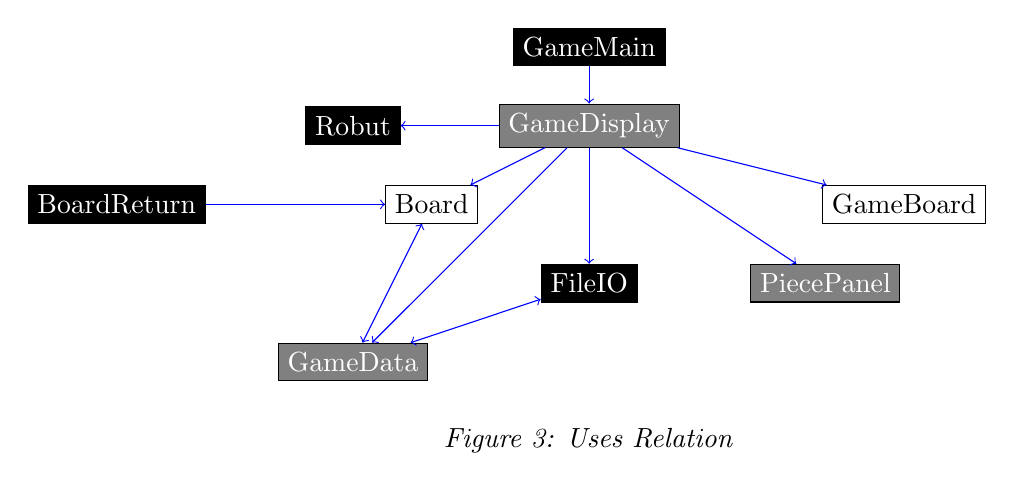
\begin{tikzpicture}
			\node[draw] (Board) at (-1,1) {Board};
			\node[draw,fill=white,text=black] (GameBoard) at (5,1) {GameBoard};
			\node[draw,fill=gray,text=white] (GameDisplay) at (1,2) {GameDisplay};
			\node[draw,fill=gray,text=white] (PiecePanel) at (4,0) {PiecePanel};
			\node[draw,fill=black,text=white] (BoardReturn) at (-5,1){BoardReturn};
			\node[draw,fill=black,text=white](GameMain) at (1,3) {GameMain};
			\node[draw,fill=gray,text=white] (GameData) at (-2,-1){GameData};
			\node[draw,fill=black,text=white] (FileIO) at (1,0) {FileIO};
			
			\node[draw,fill=black,text=white] (Robut) at (-2,2) {Robut};
			
			\draw[->,draw=blue] (GameDisplay) to (Board);
			\draw[->,draw=blue] (GameDisplay) to (PiecePanel);
			\draw[->,draw=blue] (GameDisplay) to (GameBoard);
			\draw[->,draw=blue] (BoardReturn) to (Board);
			\draw[->,draw=blue] (GameMain) to (GameDisplay);
			\draw[->,draw=blue] (GameDisplay) to (FileIO);
			\draw[->,draw=blue] (GameDisplay) to (GameData);
			\draw[<->,draw=blue] (Board) to (GameData);
			\draw[->,draw=blue] (GameDisplay) to (Robut);
			\draw[<->,draw=blue] (FileIO) to (GameData);
				\node at (1.0, -2.0) {\textit{Figure 3: Uses Relation}};
				
				\end{tikzpicture}
			\end{figure}
\noindent	In the above relation, a class points to another that it uses.\\
	GameMain only uses GameDisplay, as it only needs to create a GameDisplay object to run the program.\\ GameDisplay uses PiecePanel and Gameboard to create the panels on the window that are displayed. It uses FileIO to load and save game information to the file. It uses Board to determine game logic and apply it to the objects in the window. It uses GameData to determine the colors and what messages to display to the screen. It uses Robut to determine the actions the AI should take when playing the game. \\
	Board uses two classes BoardReturn and GameData. It uses BoardReturn to help return information to GameDisplay. It uses GameData to determine what it should tell GameDisplay to display (The controller telling the view what to do).\
	GameData uses GameDisplay, Board and FileIO. It uses these to determine what it should change in its internal variables. It represents the model of the architecture, so must interact with both the controller and the view. \\
	
	
	\newpage	
	\section{Testing}
	% A section on the testing of the software
	\subsection{Informal Black Box Testing}
	%Behavoir Table
	\begin{tabularx}{\linewidth}{|C|C|C|}
		\hline
		What was Tested & What it did & Comments \\
		\hline 
    GameControl: startboard & Printed out 'visibleteams' array & startboard is correctly setting up the 'visibleteams' array \\
    \hline 
    GameControl: startboard & Printed out "first" boolean & "first" is correctly assigned random boolean values (on 3 separate tests was assigned true, false, and false) \\
    \hline 
    GameControl: newpiece & Entered various input values (ie: 1,1,true) & Values were correctly entered into 'visibleteams' (ie: visibleteams[1][1] = 1) \\
    \hline 
    GameControl: newpiece & Was unable to place new peices in spots already occupied (ie: visibleteams[1][1] = 1, then a newpeice was entered there) & An int value of 0 was returned (meaning the move was not legal) and the array was unchanged. \\ 
    \hline 
    GameControl: movepiece & Ran function while no illegal moves attempted & Correctly returned no errors, updated array correctly \\
    \hline 
    GameControl: movepiece & Attempted to move pieces illegally on top of each other (ie: piece at [0][0] moved ontop of another piece at [0][1]) & Returned 0, no changes made to 'visibleteams' array (piece remained at [0][0], no other pieces were moved) \\
    \hline 
	\end{tabularx}
	
	\begin{tabularx}{\linewidth}{|C|C|C|}
		\hline
		What was Tested & What it did & Comments \\
		\hline 
		 GameControl: movepiece & Attempted to move pieces illegally to positions not adjacent to the current position & Returned 0, no changes made to 'visibleteams' array (piece remained at [0][0]) \\    
		 \hline 
		GameBoard: GameBoard() & Display the board, allow for color change of disks & Constructor Method for the gameboard panel. Displays the board as a set of pieces. \\
		\hline
		GameBoard: GameBoard() Change Piece Color& Pieces Change color & The display was successfully able to read in the current color array. \\
		\hline
	
		GameDisplay: GameDisplay() & Displayed panel in correct position in frame with buttons in correct positions in panel & GameDisplay is correctly setting up the panel \\
		\hline
		GameDisplay: GameDisplay()& Clicked on "New Game?" Button,  printed "New Game!" in command line & GameDisplay is correctly running through correct output for the given input \\
		\hline
		GameDisplay: GameDisplay() & Clicked on "Check!" Button, printed "Is is correct?" in command line & GameDisplay is correctly running through corect output for the given input \\
		\hline
		PiecePanel: PiecePanel() & Displayed panel in correct position in frame with circle tokens in correct position in panel & PiecePanel is correctly setting up the panel \\
		\hline
	\end{tabularx}
	\newpage
	\begin{tabularx}{\linewidth}{|C|C|C|}
		\hline
		What was Tested & What it did & Comments \\
		\hline 
		PiecePanel: PiecePanel() & Clicked on Red Circle, Displayed "add red?" & PiecePanel is giving the correct output for the given input and is ready to add a red piece to the board \\
		\hline
		PiecePanel: PiecePanel() &  Clicked on Blue Circle, Displayed "add blue?" & PiecePanel is giving the corect output for the given input and is ready to add a blue piece to the board \\
		\hline
		PiecePanel: PiecePanel()  , Clicked on Red Circle, then white circle & White Cirtcle turned red & PiecePanel is giving the corect output for the given input and should add a red piece to the board \\
		\hline
		PiecePanel: PiecePanel()  , Clicked on Red Circle, then white circle that has been coloured red & No output occurred & PiecePanel is giving the corect output for the given input and any additional red peices were not added not on their turn \\
		\hline
		PiecePanel: PiecePanel()  , Clicked on Blue Circle, then white circle that has been coloured red & The red coloured white circle turned blue & PiecePanel is giving the corect output for the given input and a blue piece should be added \\
		\hline
		PiecePanel: PiecePanel()  , Clicked on Blue Circle, then white circle & White Circle turned Blue & PiecePanel is giving the corect output for the given input and should add a blue piece to the board \\
		\hline
		PiecePanel: PiecePanel()  , Clicked on Blue Circle, then white circle that has been coloured blue & No output occurred & PiecePanel is giving the corect output for the given input and any additional red peices were not added not on their turn \\
		\hline
	\end{tabularx}
	\newpage
	\begin{tabularx}{\linewidth}{|C|C|C|}
		\hline
		What was Tested & What it did & Comments \\
		\hline 
		PiecePanel: PiecePanel()  , Clicked on Red Circle, then white circle that has been coloured blue & The blue coloured white circle turned red & PiecePanel is giving the corect output for the given input and a red piece should be added \\
		\hline
		GameDisplay & Attempted to add pieces to board & Pieces were added correctly. Game state (adding pieces) was displayed until each player had 6 pieces on board, turn system working correctly, and current turn was displayed. It was not possible to add pieces on top of each other. \\
		\hline
		GameDisplay & Attempted to move pieces across board & Pieces were only able to move to legal positions (adjacent), no flying was possible. Which players turn it was and when a piece was selected were displayed. \\
		\hline
		GameDisplay & Attempted to mill & When pieces were milled, state was displayed. Successfully deleted other players piece when mill formed. Game continued to function thereafter.\\ 
		\hline
		\end{tabularx}
		\newpage
		\begin{tabularx}{\linewidth}{|C|C|C|}
		\hline
		What was Tested & What it did & Comments \\
		\hline
		GameDisplay & Attempted to win game & When player is down to 2 pieces, the other player's winning status is displayed. \\
		\hline
		GameDisplay & Attempted to save and load game & Game saved and reloaded correctly, all pieces where they were left. \\  
		\hline
	\end{tabularx}
	\newpage
	\emph{NEW} \\
	\begin{tabularx}{\linewidth}{|C|C|C|}
		\hline 
		What was Tested & What it did & Comments \\
		\hline 
		        FileIO: saveGame and loadGame & Played partway through a game, attempted to save, exit program and continue playing & Game continued from where it was saved, all pieces remained in the same positions. \\
		        \hline 
		        Board: startboard & Printed out 'visibleteams' array & startboard is correctly setting up the 'visibleteams' array \\
		        \hline 
		        Board: startboard & Printed out "first" boolean & "first" is correctly assigned random boolean values (on 3 separate tests was assigned true, false, and false) \\
		        \hline 
		        Board: newpiece & Entered various input values (ie: 1,1,true) & Values were correctly entered into 'visibleteams' (ie: visibleteams[1][1] = 1) \\	        
		\hline
	\end{tabularx}	     
	\begin{tabularx}{\linewidth}{|C|C|C|}
		\hline 
		What was Tested & What it did & Comments \\
		\hline 
		      Board: newpiece & Was unable to place new peices in spots already occupied (ie: visibleteams[1][1] = 1, then a newpeice was entered there) & An int value of 0 was returned (meaning the move was not legal) and the array was unchanged. \\ 
		      \hline 
		      Board: movepiece & Ran function while no illegal moves attempted & Correctly returned no errors, updated array correctly \\
		      \hline 
		      Board: movepiece & Attempted to move pieces to each position on each level consecutively & Error occured. Piece was unable to move from the 7th to 0th place on level. Correction was made to identation of movepiece function. A second test of the same nature was performed, and pieces moved legally and correctly. \\
		      \hline 
		      Board: movepiece & Attempted to move pieces illegally on top of each other (ie: piece at [0][0] moved ontop of another piece at [0][1]) & Returned 0, no changes made to 'visibleteams' array (piece remained at [0][0], no other pieces were moved) \\
		      \hline 
\end{tabularx}
	\begin{tabularx}{\linewidth}{|C|C|C|}
		\hline 
		What was Tested & What it did & Comments \\
		\hline 
		      Board: checkmove & Set up board, and ran function for each piece placed & An error occured (ie: the position array [[2, 0, 0, 0, 0, 0, 1, 1], [0, 0, 0, 0, 0, 0, 0, 2]], available moves for piece in position [0][0] : [[0, 1, 0, 0, 0, 0, 0, 1], [0, 0, 0, 0, 0, 0, 0, 0]] ) Correction to checkmove made. Test repeated, successful. \\
		      \hline 
		      Board: okaymovecheck & Set up board, when team had an available move & Returned a 1, test successful. \\
		      \hline 
		      Board: okaymovecheck & Set up board, when team had no available move & Returned a 0, test successful. \\
		      \hline 
		      Board: movepiece, checkpiece & Attempted to move pieces illegally to positions not adjacent to the current position & Returned 0, no changes made to 'visibleteams' array (piece remained at [0][0]) \\   
		      \hline 
	\end{tabularx}
	
		\begin{tabularx}{\linewidth}{|C|C|C|}
			\hline 
			What was Tested & What it did & Comments \\
			\hline 
			GameDisplay: Starting a game against an AI & A game began and one of the players was controlled by the game & This was the expected result. \\ \hline 
			robut: place(), with input visibleTeams = {{0,0,2,0,0,0,1,1}, {0,0,0,0,0,0,0,0}} , 1 , 3 & Output location was 0,0 & Place() is functioning correctly \\ \hline 
			robut: place(), with input visibleTeams = {{0,0,2,0,0,0,1,1}, {0,0,0,0,0,0,0,0}} , 2 , 3 & Output location was 0,0 &Place() is functioning correctly \\ \hline 
			robut: place(), with input visibleTeams = {{0,0,2,0,0,0,0,0}, {0,0,0,0,0,2,1,2}} , 1 , 2 & The function got stuck in an infinite loop & Changed randomAdjacent() so it does not randomly select a piece but instead it uses a for loop to check for a piece with and adjacent empty space \\ \hline 
			robut: place(), with input visibleTeams = {{0,0,2,0,0,0,0,0}, {0,0,0,0,0,2,1,2}} , 1 , 2 & Array out of bound exception & Changed randomAdjacent() so it either returns an array of the location or it returns null \\ 	
			 \hline 
		\end{tabularx}	
			\begin{tabularx}{\linewidth}{|C|C|C|}
				\hline 
				What was Tested & What it did & Comments \\
				\hline 
				robut: place(), with input visibleTeams = {{0,0,2,0,0,0,0,0}, {0,0,0,0,0,2,1,2}} , 1 , 2 & Output location was {0,4} & Place() is functioning correctly \\ \hline 
				robut: move(), with input visibleTeams = {{0,1,2,1,0,2,2,2}, {0,1,1,2,0,0,0,0}} , 2 & Output piece and location were {0,7} and {0,0} & Move is not functioning correctly, added catch so pieces in near mills cannot move to try complete themselves \\ \hline 
				robut: move(), with input visibleTeams = {{0,1,2,1,0,2,2,2}, {0,1,1,2,0,0,0,0}} , 2 & Output piece and location were {1,3} and {1,4} & Move is functioning correctly \\ \hline 
				robut: move(), with input visibleTeams = {{0,1,2,1,0,2,2,2}, {0,1,1,2,0,0,0,0}} , 1 & Output piece and location were {0,1} and {0,0} & Move is functioning correctly \\ \hline \\
				robut: mill(), with input visibleTeams = {{0,1,2,1,0,2,2,2}, {0,1,1,2,0,0,0,0}} , 1 & Output was {0,6} & Mill is functioning correctly \\
				 \hline 
				\end{tabularx}
	\begin{tabularx}{\linewidth}{|C|C|C|}
		\hline 
		What was Tested & What it did & Comments \\
		\hline 
		robut: mill(), with input visibleTeams = {{0,1,2,1,0,2,2,2}, {2,1,1,2,0,0,0,0}} , 1 & Output was {0,0} & Mill is functioning correctly \\ \hline 
		Board was {{2,1,2,1,2,0,2,1}, {0,1,2,1,2,0,1,0}}, piece at 0,7 was clicked and was attempted to be moved to 1,7 & Piece could not be moved to 1,7. Random clicking led to the piece finally being moved to 1,0 & Game is not functioning correctly \\ \hline 
		Playing game with AI, Board was {{1,0,2,2,2,0,1,2} {1,1,2,0,1,1,2,1}}, player (2) has mill and tried to remove a 1 piece & Piece could not be removed, blue got an extra turn & Game is not functioning correctly \\
		\hline 
		Playing game with AI, Board was {{1,0,2,2,0,2,1,2} {1,1,2,0,1,1,2,1}}, player (2) moved piece at 0,5 to 0,4 to create mill & Game did not recognize mill, instead game was ended in draw & Game is not functioning correctly \\ \hline 
		Playing game with AI, Board was {{0,0,1,2,1,1,1,0} {2,1,1,2,2,0,0,2}}, computer (1) has mill & AI did not remove piece, instead got an extra turn to move & Game is not functioning correctly \\ 
		\hline 
		\end{tabularx}	
		\section{Computer Player AI}	
		\indent The computer player was designed with the three states of gameplay in mind. Just as the player was implemented through parsing inputs in differing methods depending on the state of the game, the computer was implemented as an abstract class that returns inputs of where to move next depending on which state the game is in. For each state there is a corresponding function to determine what move the computer player should make: place() corresponds with state 1; move() corresponds with state 2; mill() corresponds with state 3.\\
		The computer player was designed with the three states of gameplay in mind. Just as the player was implemented through parsing inputs in differing methods depending on the state of the game, the computer was implemented as an abstract class that returns inputs of where to move next depending on which state the game is in. For each state there is a corresponding function to determine what move the computer player should make: place() corresponds with state 1; move() corresponds with state 2; mill() corresponds with state 3.\\
		The function move() works in a similar fashion. It begins by checking if the computer has a near mill. If it has that it continues to check for whether there is one of the computer’s pieces adjacent to the empty spot of the near mill. If that is true, then the piece is moved to complete the mill. However, if any one of those are false move() checks if the other player has a near mill. If true, it continues to check for whether one of the computer’s pieces is adjacent to the empty spot of the opponent’s near mill. If that is also true, the piece is moved to block the other player from creating a mill. If all else fails, a random piece of the computer’s is moved to a random open adjacent location.\\
		Finally, mill()’s implementation follows that of move() and place(). It begins by checking if the opposing player has a mill and, if it does, randomly removes one of the three pieces that make up the mill. If the opponent does not have a mill, the function checks if they have a near mill instead and removes one of the pieces that makes it up, if it exists. Otherwise, mill() randomly removes one of the opponent’s pieces.\\		
	\section{Discussion}
	%4.6 Internal review/ evaluation of design
	The design follows the MVC format quite well. The model is implemented in GameData; the View is implemented in GameBoard, PiecePanel, and GameDisplay; and the Controller is implemented in Main and Board. Each class is much better balanced in terms of the tasks it should be doing and how it is interacting with the other classes, as compared to assignment 2. The code is properly modularized to follow MVC format and there is a clear hierarchy. The group would give this project an 8/10 due to the improvements made.
	
	\subsection{Anticipated Changes}
	% what was designed in anticipation of changes
	\begin{itemize}
	\item Board: In the future, should any additional rules be implemented in the game, it would not be difficult to integrate them with the already exsisting ones.  
	Additionally, the Board could be easily used with different dimensions (ie: 8 Men's Morris).  
	\item    Boardreturn: Class designed to hold variables needed to determine whether a move/new piece is legal. Returns a integer indicating the legality, and a int[][], indicating the current board array. Due to the design of a separate type to bundle this data, if any other data feedback is required in the future, it will be simple to add it in.
	\item FileIO: In the future, the program could store additional data from the user (high score, trends, etc), by writing it to the .txt file.
	
	\end{itemize}
	
\end{document}